%!TEX program = xelatex
\documentclass[10pt]{article}
\usepackage{amssymb}
\usepackage{amsmath}
\usepackage{mathrsfs}
\usepackage{titlesec}
\usepackage{xcolor}
%\usepackage[shortlabels]{enumitem}
\usepackage{enumerate}
\usepackage{bm}
\usepackage{tikz}
\usepackage{listings}
\usetikzlibrary{arrows}
\usepackage{subfigure}
\usepackage{graphicx,booktabs,multirow}
\usepackage[a4paper]{geometry}
\usepackage{upquote}
\usepackage{float}
\usepackage{pdfpages}

\usepackage[colorlinks,linkcolor=blue]{hyperref}
\usepackage{mdframed}

\iffalse
\usepackage{lastpage}
\usepackage{fancyhdr}
\fancyfoot[C]{Page \thepage\ of \pageref{LastPage}}
% Uncomment to remove the header rule
\renewcommand{\headrulewidth}{0pt} 
\pagestyle{fancy}
\fi

\geometry{verbose,tmargin=2cm,bmargin=2cm,lmargin=2cm,rmargin=2cm}
\geometry{verbose,tmargin=2cm,bmargin=2cm,lmargin=2cm,rmargin=2cm}
\lstset{language=Matlab}
\lstset{breaklines}

\input defs.tex

\newenvironment{solution}
    { \begin{mdframed}[backgroundcolor=gray!10] \textcolor{cyan}{\textbf{Solution}} \\}
    {  \end{mdframed}}

\newtheorem{proposition}{Proposition}
\newtheorem{remark}{Remark}

\titleformat*{\section}{\centering\LARGE\scshape}
\renewcommand{\thesection}{\Roman{section}}
\lstset{language=Matlab,tabsize=4,frame=shadowbox,basicstyle=\footnotesize,
keywordstyle=\color{blue!90}\bfseries,breaklines=true,commentstyle=\color[RGB]{50,50,50},stringstyle=\ttfamily,numbers=left,numberstyle=\tiny,
  numberstyle={\color[RGB]{192,92,92}\tiny},backgroundcolor=\color[RGB]{245,245,244},inputpath=code}

\begin{document}

%\title{CS150: Database and Data Mining \\%
%	Final Exam}
%\maketitle


\section{Basics \textbf{[10 points]}}
For each image on the next page, select the letter corresponding to the best description. \\
A. Left Deep Tree \\
B. Key Compression \\
C. B+ Tree \\
D. ISAM \\
E. Nested Loops Join \\
F. Sort Merge Join \\
G. Indexed Nested Loop Join \\
H. Slotted Page \\
I. Variable Length Tuple \\
J. Fixed Length Tuple \\
K. Buffer Frame \\
L. Sort based group by \\
M. mapPartitions \\
N. Tournament Sort \\
%\newpage
\begin{figure}
	\centering
	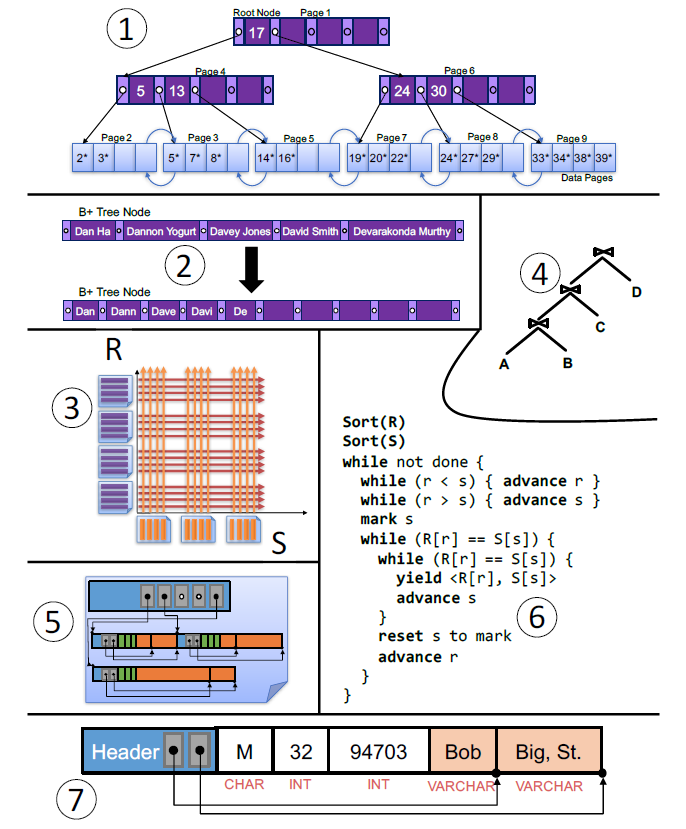
\includegraphics[width=.9\linewidth]{basics.png}
\end{figure}


\newpage
\section{SQL and ER Modeling \textbf{[12 points]}}
\begin{enumerate}

	\item \textbf{[2 points]}
	      Which of the following expressions computes the matrix vector product:
	      $$
		      (\mathbf{A} \mathbf{x})_{i}=\sum_{k=1}^{d} A_{i k} x_{k}
	      $$
	      Assume $\mathbf{A}$ and $\mathbf{x}$ have compatible dimensions and there is only one correct answer.\\
	      A.
	      \begin{lstlisting}
SELECT A.row AS row, A.value * x.value AS value 
FROM A JOIN x
ON A.row = x.row
\end{lstlisting}
	      B.
	      \begin{lstlisting}
SELECT A.row AS row, SUM(A.value * x.value) AS value 
FROM A JOIN x
ON A.row = x.row
GROUP BY A.col
\end{lstlisting}
	      C.
	      \begin{lstlisting} 
SELECT x.row AS row, SUM(A.value * x.value) AS value 
FROM A JOIN x
ON A.col = x.row
GROUP BY A.col
\end{lstlisting}
	      D.
	      \begin{lstlisting} 
SELECT A.row AS row, SUM(A.value * x.value) AS value 
FROM A JOIN x
ON A.col = x.row
GROUP BY A.row
\end{lstlisting}

	\item \textbf{[2 points]}
	      Suppose we wanted to compute the element-wise sum of the vectors $\mathbf{x}$
	      and $\mathbf{y}$ using the SQL expression:
	      \begin{lstlisting}
SELECT x.row AS row, SUM(x.value + y.value) AS value 
FROM x JOIN y 
ON x.row = y.row
\end{lstlisting}
	      Which of the following statements about this query are true?
	      (You may mark zero ($\phi$), one or more than one of the choices.)\\
	      A. Some non-zero entries may be omitted from the final result.\\
	      B. The correct query should use LEFT OUTER JOIN.\\
	      C. The correct query should use FULL OUTER JOIN.\\
	      D. There is nothing wrong.

	\item \textbf{[8 points]}
	      There are four tables. SALESPERSON contains the names, ids \& quotas for the salespeople, and names are not unique.
	      PRODUCTS contains the product names, product ids, and prices for the products.
	      The product ids are unique.
	      CUSTOMERS contains the customer names, customer ids, and regions for the customers (customer ids are unique),
	      and ORDERS contains the customer id, the product id, and the product ordered per customer.\\
	      \begin{center}
		      \begin{tabular}{|l|l|l|}
			      \multicolumn{2}{c} { SALESPERSON }     \\
			      \hline Sname          & Sid & Quota    \\
			      \hline Frances        & 25  & $\$ 100$ \\
			      \hline $\mathrm{Bob}$ & 31  & $\$ 150$ \\
			      \hline Frances        & 74  & $\$ 200$ \\
			      \hline Mary           & 89  & $\$ 250$ \\
			      \hline
		      \end{tabular} \qquad
		      \begin{tabular}{|l|l|l|}
			      \multicolumn{2}{c} { PRODUCTS }  \\
			      \hline Pname    & Pid & Pprice   \\
			      \hline disks    & 131 & $\$ 100$ \\
			      \hline pcs      & 152 & $\$ 700$ \\
			      \hline macs     & 831 & $\$ 800$ \\
			      \hline printers & 255 & $\$ 120$ \\
			      \hline paper    & 221 & $\$ 5$   \\
			      \hline
		      \end{tabular} \\
		      \begin{tabular}{|l|l|l|}
			      \multicolumn{2}{l} { CUSTOMERS } \\
			      \hline Cname  & Cid & Region     \\
			      \hline Bob    & 1   & TX         \\
			      \hline Harry  & 2   & TX         \\
			      \hline Lin    & 3   & MA         \\
			      \hline Martha & 4   & FL         \\
			      \hline Lin    & 5   & FL         \\
			      \hline Leyla  & 6   & CA         \\
			      \hline
		      \end{tabular} \qquad
		      \begin{tabular}{|l|l|l|}
			      \multicolumn{3}{c} { ORDERS } \\
			      \hline Cid & Pid & Quantity   \\
			      \hline 1   & 152 & 1          \\
			      \hline 2   & 152 & 1          \\
			      \hline 4   & 831 & 1          \\
			      \hline 4   & 131 & 1          \\
			      \hline 5   & 255 & 1          \\
			      \hline 6   & 831 & 1          \\
			      \hline
		      \end{tabular}
	      \end{center}
	      \begin{itemize}
		      \item[(a)] \textbf{[2 points]} Select the true SQL expression(s) for “List the names of the customers who have bought more than one item.”
		            (You may mark zero ($\phi$), one or more than one of the choices.)\\
		            A.\begin{lstlisting}
	SELECT cname
	FROM customers
	WHERE cid IN (SELECT cid
	              FROM orders
	              GROUP BY cid
	              HAVING count(*) > 1)
\end{lstlisting}
		            B.\begin{lstlisting}
	SELECT c.cname
	FROM customers c, (SELECT cid  
	                   FROM orders
	                   GROUP BY cid
	                   HAVING count(*) > 1) as o
	WHERE c.cid = o.cid
\end{lstlisting}
		            C. \begin{lstlisting}
	SELECT cname
	FROM customers
	WHERE (SELECT count(*)
	       FROM orders
	       GROUP BY pid ) > 1
\end{lstlisting}
		            D. \begin{lstlisting}
	SELECT cname
	FROM customers c, orders o1, orders o2
	WHERE c.cid = o1.cid and c.cid = o2.cid and o1.cid < > o2.pid
\end{lstlisting}

		      \item[(b)] \textbf{[2 points]} Select the true SQL expressions for “List the names, pid, and price of all the products, whether or not the product has been ordered,
		            but if it has been ordered by the cids of the customer who ordered it.”
		            (You may mark zero ($\phi$), one or more than one of the choices.)\\
		            A. \begin{lstlisting}
	SELECT name, pid, price, cid
	FROM products LEFT OUTER JOIN orders
\end{lstlisting}
		            B. \begin{lstlisting}
	SELECT name, pid, price, cid 
	FROM products LEFT OUTER JOIN orders
	ON products.pid = orders.pid
\end{lstlisting}
		            C. \begin{lstlisting}
	SELECT name, p.pid, price, cid
	FROM products p, orders o
	WHERE p.pid = o.pid
	UNION
	SELECT name, pid, price
	FROM products p
	WHERE NOT EXISTS (SELECT * FROM orders o WHERE o.pid = p.pid)
\end{lstlisting}
		            D. \begin{lstlisting}
	SELECT name, p.pid, price, cid
	FROM products p, orders o
	WHERE p.pid = o.pid
	UNION
	SELECT name, pid, price, NULL as cid
	FROM products p
\end{lstlisting}

		      \item[(c)] \textbf{[4 points]}
		            Now, let's complete the ER diagram with the tables given above and some new translations.
		            You need to underline the primary keys, add arrows. If bolding a line/arrow,
		            be sure to clearly make it bold. If here's weak entity, also be sure to clearly show it.\\
		            •	Each product sold by exactly one salesperson.\\
		            •	The sid of salesperson in the same shop is unique, however two salesperson in different shop might have the same sid.\\
		            •	A salesperson can only work in one shop.\\
		            •	The address can uniquely identify a shop.\\
		            \begin{figure}[ht]
			            \centering
			            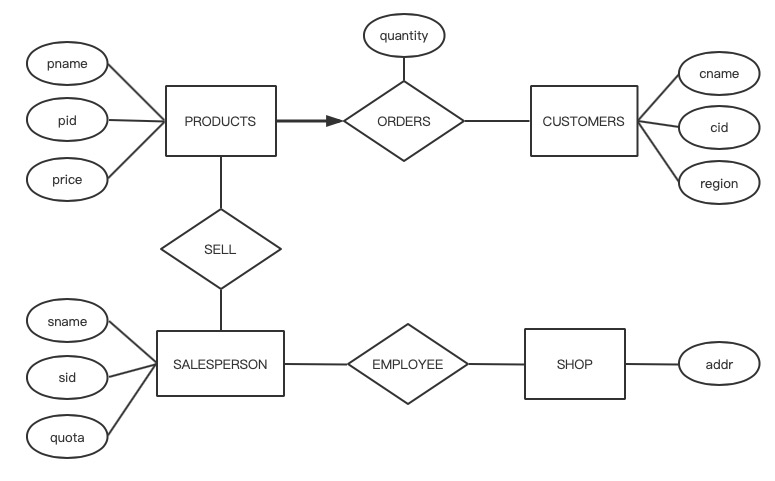
\includegraphics[width=0.7\linewidth]{E_R}
		            \end{figure}
	      \end{itemize}
\end{enumerate}


\newpage
\section{Indexes and B+ Trees \textbf{[9 points]}}

\begin{enumerate}

	\item \textbf{[5 points]} Basics of B+ Trees.
	      \begin{itemize}
		      \item[(a)] \textbf{[1 point]} What is the maximum fan out $F$ of an order $d$ B+ tree? %\underline{\hbox to 20mm{}}

		      \item[(b)] \textbf{[2 points]}
		            Assume that each leaf can hold $F$ data entries. What is the maximum number of data entries
		            that an order $d$ B+ tree of height 5 can store? Express your answer as a function of $F$. (Note that a height 1 B+ tree only has a root node).

		      \item[(c)] \textbf{[2 points]}
		            Again, assume that each leaf can hold $F$ data entries. And we have indexed a file with $1\times 10^9$ records with this
		            order $d$ B+ tree. What is the minimum number of I/Os it will take to check if a data entry exists in this tree?
		            Express your answer as a function of $F$.
	      \end{itemize}

	\item \textbf{[4 points]}
	      Consider the following B+ tree of order 2.
	      \begin{center}
		      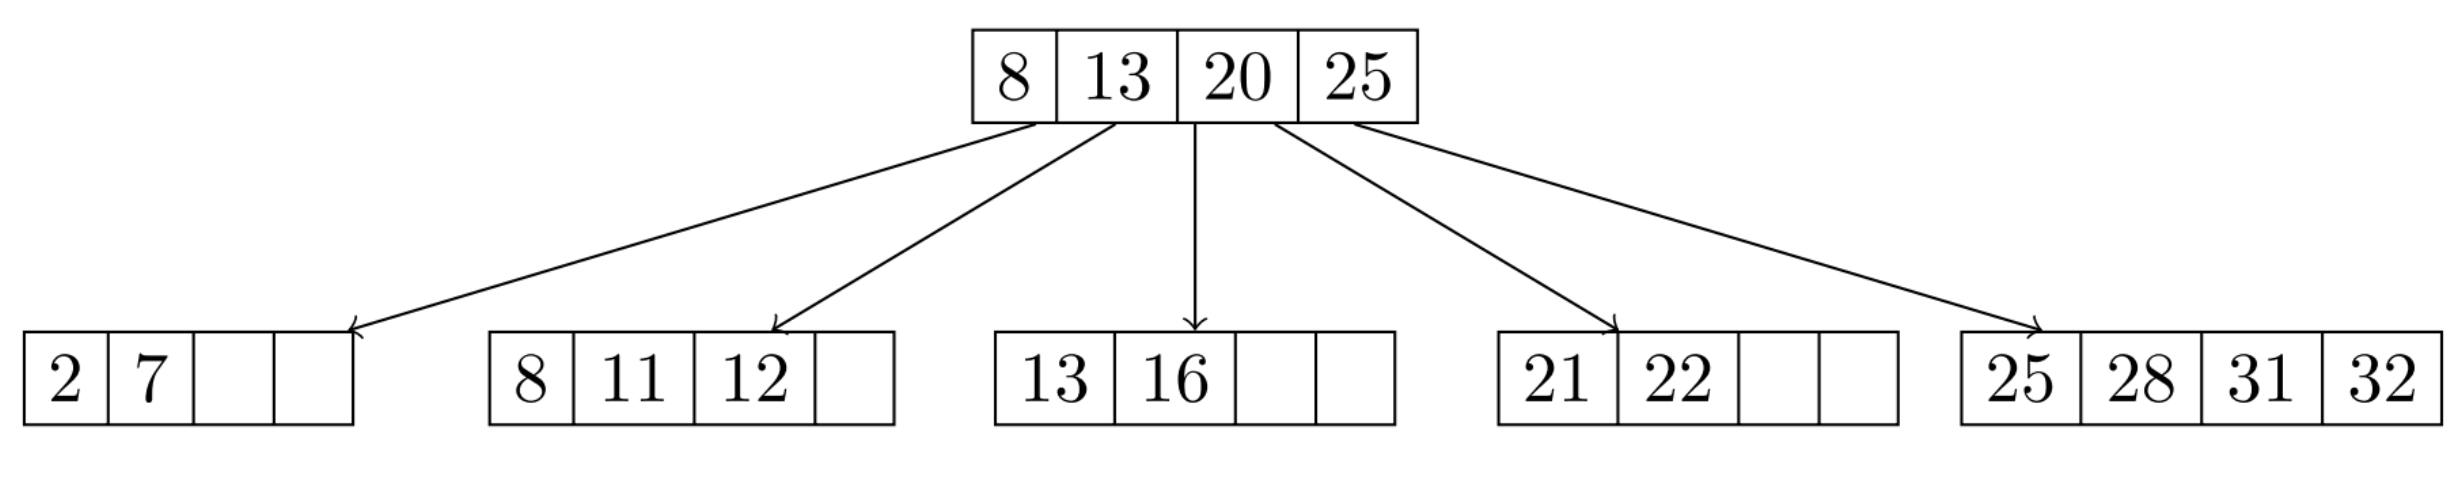
\includegraphics[scale=0.25]{Btree.png}
	      \end{center}
	      \begin{itemize}
		      \item[(a)] \textbf{[1 point]} How many nodes split when you insert 27?

		      \item[(b)] \textbf{[1 point]} After inserting 27 into the tree, you also insert 26. How many nodes split as a result of inserting
		            26?

		      \item[(c)] \textbf{[2 points]} Assume that after inserting 26 and 27, you insert the keys 34, 35, 36, . . ., 100. After all these
		            insertions, what keys are in the leftmost leaf node?
	      \end{itemize}
\end{enumerate}


\newpage
\section{External Sorting \textbf{[8 points]}}
\begin{enumerate}
	\item \textbf{[2 points]} True or False:
	      \begin{itemize}
		      \item[(a)] Increasing the number of buffer pages don't affects the number of I/Os performed in Pass 0 of an external sort.
		      \item[(b)] Double buffering reduces the time it takes to sort records within a single page.
	      \end{itemize}

	\item \textbf{[6 points]}
	      Assume that each page is 4 KB large, and that you have a 24KB buffer pool (with 6 frames).
	      \begin{itemize}
		      \item[(a)] \textbf{[2 points]} How many passes would it take to externally sort an 512KB file?
		            Include the initial sorting pass and subsequent merging passes in your answer. You need to simplify your answer.
		      \item[(b)] \textbf{[2 points]} What would be the total cost in I/Os for this external sort?
		      \item[(c)] \textbf{[2 points]} What is the minimum number of additional buffer frames we require to reduce the number of passes
		            (from part 1) by 1? %You do not need to simplify your answer.
		            %	\item[(c)] \textbf{[2 points]} In order to sort the file in two passes, how many additional buffer pages are necessary?
	      \end{itemize}
\end{enumerate}


\newpage
\section{Join Algorithms \textbf{[8 points]}}

\begin{enumerate}
	\item \textbf{[5 points]}
	      Consider a relation R with attributes $(x,y)$ and a relation S with attributes $(y, z)$.
	      Column $y$ in S is a key and the set of values of $y$ in R are the same as the set of values of $y$ in S.
	      Assume that there are no indexes available and that there are 25 pages in the buffer available.
	      Table R is 1,500 pages with 50 tuples per page. Table S is 400 with 100 tuples per page.
	      Compute the I/O costs for the following joins. Assume the simplest cost model, where pages are read and written one at a time.
	      \begin{itemize}
		      \item[(a)] \textbf{[1 point]} Block nested loops join with R as the outer relation and S as the inner relation.
		      \item[(b)] \textbf{[1 point]} Block nested loops join with S as the outer relation and R as the inner relation.
		      \item[(c)] \textbf{[1 point]} Sort merge join with R as the outer relation and S as the inner relation.
		      \item[(d)] \textbf{[1 point]} Sort merge join with S as the outer relation and R as the inner relation.
		      \item[(e)] \textbf{[1 point]} Hash join with S as the outer relation and R as the inner relation.
	      \end{itemize}

	\item \textbf{[3 points]}
	      Consider a new case, i.e. B>4 pages worth of buffer space, and relations M and N of size > B.
	      Please fill the blanks below with ``always'', ``sometimes'' or ``never''.
	      \begin{itemize}
		      \item[(a)] \textbf{[1 point]} Block nested loop join is \underline{\ \ \ \ \ \ \ \ \ \ } better than page-oriented nested loop join.
		      \item[(b)] \textbf{[1 point]} Sort-merge join is \underline{\ \ \ \ \ \ \ \ \ \ } better than hash-join.
		      \item[(c)] \textbf{[1 point]} Hybrid Hash-Join is \underline{\ \ \ \ \ \ \ \ \ \ } better than block-nested loops join.
	      \end{itemize}
\end{enumerate}

%\newpage
%\section{Buffer Manager}


\newpage
\section{Query Optimization \textbf{[10 points]}}
%\subsection{Selectivity Estimation}
Consider two relations Cat(age, weight, price) and Pocket(money), with 150 tuples and 100 tuples respectively.
We have an index on Cat.age with 15 unique integer values uniformly distributed in the range [1, 15],
an index on Cat.weight with 30 unique float values uniformly distributed in the range [2001, 5000],
an index on Cat.price with 10 unique integer values uniformly distributed in the range [11, 20],
and an index on Pocket.money with 15 unique integer values uniformly distributed in the range [11, 25]. \\
%We do not have an index on Cat.price.\\
Use selectivity estimation to estimate the number of tuples produced by the following queries.
\begin{itemize}
	\item[(a)] \textbf{[1 point]} SELECT * FROM Cat\\
	\item[(b)] \textbf{[2 points]} SELECT * FROM Cat WHERE age $\geq$ 10\\
	\item[(c)] \textbf{[2 points]} SELECT * FROM Cat WHERE age $\textless$ 5 AND weight $\leq$ 3000\\
	\item[(d)] \textbf{[2 points]} SELECT * FROM Cat WHERE age $\textgreater$ 10 OR price $\geq$ 15\\
	\item[(e)] \textbf{[3 points]} SELECT * FROM Cat, Pocket WHERE Cat.price = Pocket.money\\
\end{itemize}



\newpage
\section{Transaction and Concurrency \textbf{[10 points]}}
%\href{https://drive.google.com/file/d/1Dzza4FvIVK17h_VdYF4M-TD5f-CnIY95/view}{Link to the reference}\\
Consider the following schedule. (For each of the questions below, you may mark zero ($\phi$), one
or more than one of the choices.)
\begin{center}
	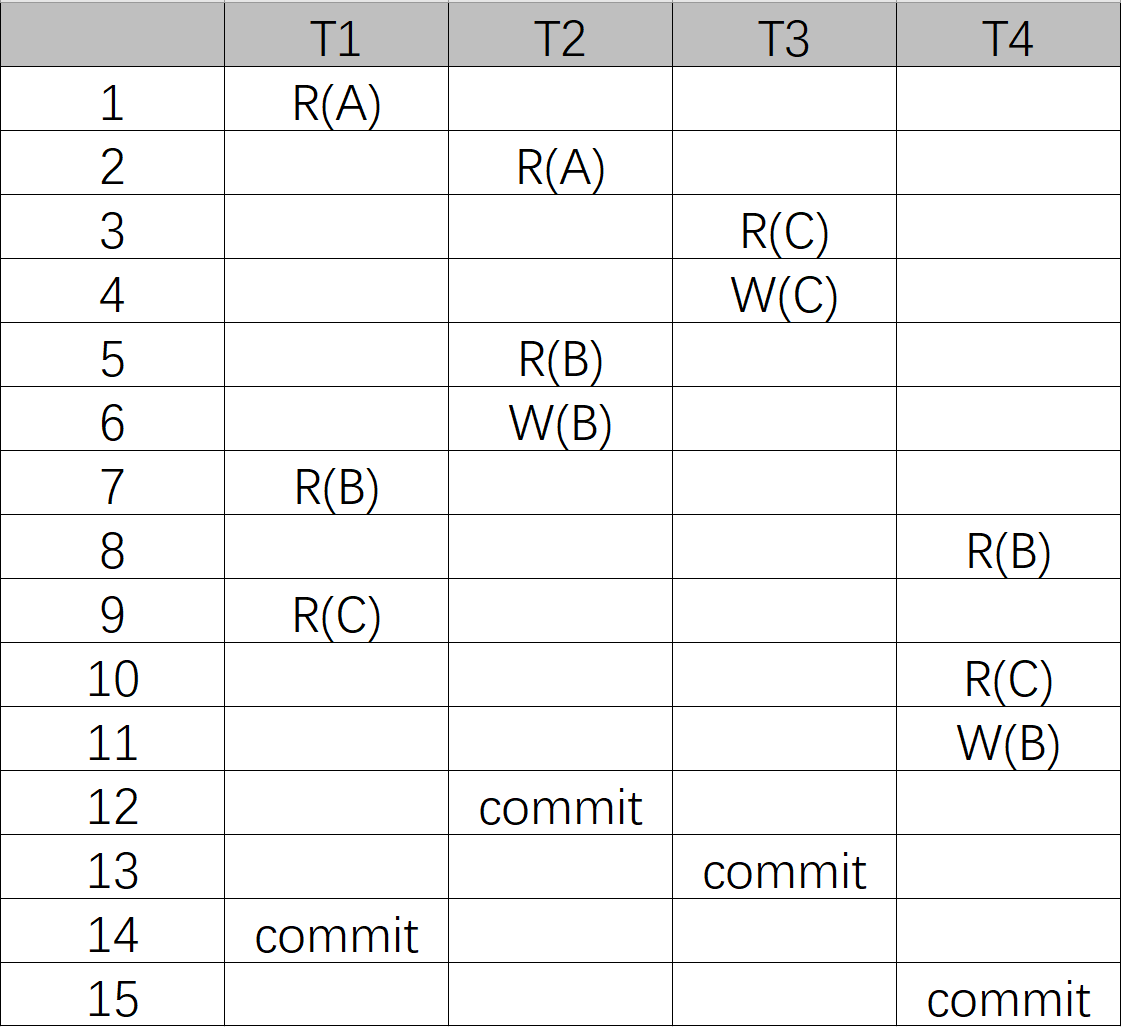
\includegraphics[scale=0.35]{transaction.png}
\end{center}
\begin{itemize}
	\item[(a)] \textbf{[1 point]} What transactions is T1 pointing to in the conflict graph for the schedule above?\\
	      A. T1\\
	      B. T2\\
	      C. T3\\
	      D. T4

	\item[(b)] \textbf{[1 point]} What transactions is T2 pointing to in the conflict graph for the schedule above?\\
	      A. T1\\
	      B. T2\\
	      C. T3\\
	      D. T4

	\item[(c)] \textbf{[1 point]} What transactions is T3 pointing to in the conflict graph for the schedule above? \\
	      A. T1\\
	      B. T2\\
	      C. T3\\
	      D. T4

	\item[(d)] \textbf{[1 point]} What transactions is T4 pointing to in the conflict graph for the schedule above? \\
	      A. T1\\
	      B. T2\\
	      C. T3\\
	      D. T4

	\item[(e)] \textbf{[3 points]} Which of the following locking disciplines could have produced the above schedule?\\
	      A. 2 phase locking\\
	      B. Strict 2 phase locking

	\item[(f)] \textbf{[3 points]} Which of the following schedules below are conflict equivalent to the schedule above?\\
	      A. T3, T1, T2, T4\\
	      B. T2, T3, T1, T4\\
	      C. T4, T3, T1, T2\\
	      D. T1, T2, T3, T4\\
	      E. T3, T2, T1, T4

\end{itemize}


\newpage
\section{Logging and Recovery \textbf{[13 points]}}
\begin{enumerate}
	\item \textbf{[5 points]} \textbf{General Logging and Recovery.} \\
	      Mark the boxes for all true statement(s):
	      \begin{itemize}
		      \item[(a)] Schedules produced by two phase locking are guaranteed to prevent cascading aborts.
		      \item[(b)] Strict two phase locking is both necessary and sufficient to guarantee conflict serializability.
		      \item[(c)] In a system that uses strict two-phase locking, if a transaction aborts, it releases all of its locks as soon as rollback is complete.
		      \item[(d)] In a system that uses strict two-phase locking, a transaction that only performs reads can never enter a deadlock cycle.
		      \item[(e)] When aborting a transaction, it is necessary to modify pages on disk.
		      \item[(f)] During recovery, the ARIES protocol redo aborted transactions.
		      \item[(g)] When a transaction commits, any modified buffer pages must be written to durable storage.
		      \item[(h)] In ARIES recovery, after the analysis phase, the recLSN of each page in the dirty page table must be larger than the pageLSN of the corresponding page.
		      \item[(i)] If PageLSN is greater than the max LSN flushed so far (flushedLSN), we can safely write this page to disk.
		      \item[(j)] Write-Ahead Logging (WAL) guarantees that a transactions log records are flushed to disk before the transaction commit.
	      \end{itemize}

	\item \textbf{[8 points]} \textbf{Recovery.} \\
	      Your database server has just crashed due to a power outage.
	      You boot it back up, find the following log and checkpoint information on disk,
	      and begin the recovery process. Assume we use a STEAL/NO FORCE recovery policy.
	      \begin{figure}[h]
		      \centering
		      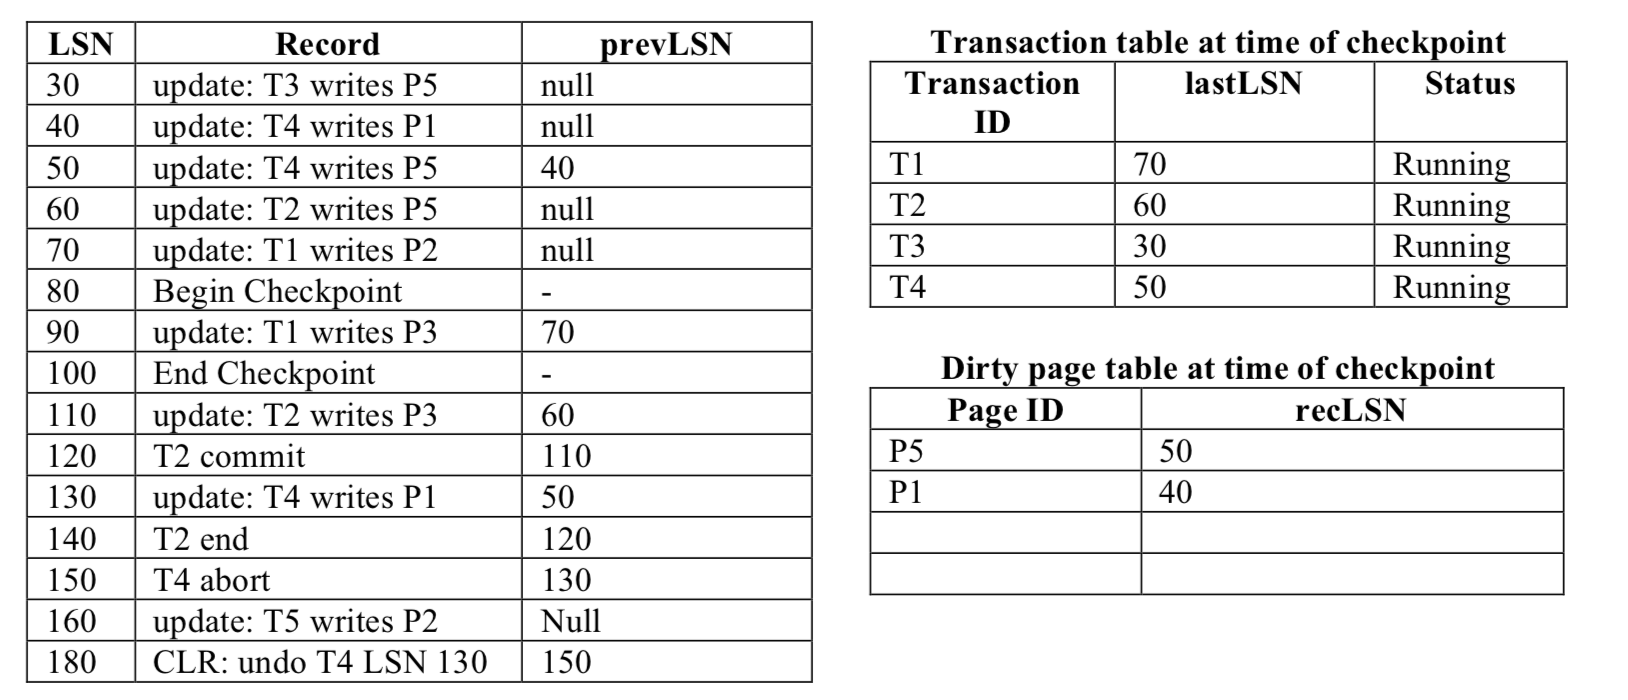
\includegraphics[width=\linewidth]{recovery}
		      %	\caption{Logging and recovery}
		      \label{fig:recovery}
	      \end{figure}
	      \begin{itemize}
		      \item[(a)] \textbf{[2 points]}
		            At the end of the Analysis phase, what transactions will be in the transaction table,
		            and with what lastLSN and Status values?
		            \begin{table}[h]
			            \centering
			            \begin{tabular}{|c|c|c|}
				            \hline
				            Transaction ID & lastLSN & status \\
				            \hline
				                           &         &        \\
				            \hline
				                           &         &        \\
				            \hline
				                           &         &        \\
				            \hline
				                           &         &        \\
				            \hline
			            \end{tabular}
			            \caption{Transaction table}
		            \end{table}
		      \item[(b)] \textbf{[2 points]}
		            At the end of the Analysis phase, what pages will be in the dirty page table, and with what recLSN values?
		            \begin{table}[h]
			            \centering
			            \begin{tabular}{|c|c|}
				            \hline
				            page ID & recLSNs \\
				            \hline
				                    &         \\
				            \hline
				                    &         \\
				            \hline
				                    &         \\
				            \hline
				                    &         \\
				            \hline
			            \end{tabular}
			            \caption{Dirty page table}
		            \end{table}

		            \iffalse
			            \begin{table}[h]
				            \parbox{.45\linewidth}{
					            \centering
					            \begin{tabular}{|c|c|c|}
						            \hline
						            Transaction ID & lastLSN & status \\
						            \hline
						                           &         &        \\
						            \hline
						                           &         &        \\
						            \hline
						                           &         &        \\
						            \hline
						                           &         &        \\
						            \hline
					            \end{tabular}
					            \caption{transaction table}
				            }
				            \hfill
				            \parbox{.45\linewidth}{
					            \centering
					            \begin{tabular}{|c|c|}
						            \hline
						            page ID & recLSNs \\
						            \hline
						                    &         \\
						            \hline
						                    &         \\
						            \hline
						                    &         \\
						            \hline
						                    &         \\
						            \hline
					            \end{tabular}
					            \caption{dirty page table}
				            }
			            \end{table}
		            \fi

		      \item[(c)] \textbf{[4 points]} At which LSN in the log should redo begin? Which log records will be redone (list their LSNs)?
	      \end{itemize}
\end{enumerate}


\newpage
\section{Data Mining and Machine Learning \textbf{[20 points]}}

\begin{enumerate}

	\item \textbf{[4 points]} \textbf{General Data Mining and Machine Learning.} \\
	      Mark the boxes for all true statement(s):
	      \begin{itemize}
		      \item[(a)] In multi-dimensional data model, it contains one fact table and multiple dimension tables.
		      \item[(b)] The order of the basic KDD (Knowledge Discovery in Database) process is Data Selection, Data Cleaning, Evaluation, Data Mining \& ML.
		      \item[(c)] In supervised machine learning labeled data is used to train a model.
		      \item[(d)] Classification models would be a good candidate when trying to predict the total
		            amount of time a user spends browsing a page.
		      \item[(e)] The ultimate goal in machine learning is to find a model that best fits the training data.
		      \item[(f)] The $k$-means algorithm is guaranteed to converge to the global optimum.
		      \item[(g)] The bag-of-words model encodes text as a vector.
		      \item[(h)] A common form of feature engineering on continuous data is one-hot-encoding.
	      \end{itemize}

	\item \textbf{[8 points]} \textbf{K-Means.}
	      \begin{itemize}
		      \item[(a)] \textbf{[2 points]} True or False: \\
		            %A. No matter which points are selected as the initial cluster centers, the K-means algorithm is guaranteed to converge to the global optimum.\\
		            Suppose we are going to cluster the following dataset: $\{(x_1, y_1), ..., (x_n, y_n)\}$,
		            denote $\Bar{x} = \frac{1}{n}\sum_{i=1}^n x_i$ and $\Bar{y} = \frac{1}{n}\sum_{i=1}^n y_i$,
		            we can have a decentralized dataset $\{(x_1', y_1'), ..., (x_n', y_n')\}$
		            where $x_i' = x_i - \Bar{x}$, $y_i' = y_i - \Bar{y}$, $i = 1,2,...,n$.
		            The $k$-means algorithm will converge to the same result if we choose the initial
		            centers as $\{(x_s, y_s), (x_t, y_t)\}$ for the original dataset and $\{(x_s', y_s'), (x_t', y_t')\}$
		            for the decentralized dataset, where $s, t$ are two different constants.

		      \item[(b)] \textbf{[2 points]}
					Which of the following can act as possible termination conditions in $k$-means?
					(you may mark zero ($\phi$), one or more than one of the choices.)\\
		            A. For a fixed number of iterations.\\
		            B. Assignment of observations to clusters does not change between iterations. Except for cases with a bad local minimum.\\
		            C. Centroids do not change between successive iterations.\\
		            D. Terminate when RSS falls below a threshold.\\


		      \item[(c)] \textbf{[2 points]}
					In which of the following cases will $k$-means clustering fail to give good results? 
					(you may mark zero ($\phi$), one or more than one of the choices.)\\
		            A. Data points with outliers.\\
		            B. Data points with different densities.\\
		            C. Data points with round shapes.\\
		            D. Data points with non-convex shapes.\\

		      \item[(d)] \textbf{[2 points]}
		            The following is a set of one-dimensional points: $\{-4, 0, 1, 2, 3, 5, 7, 10, 13, 22\}$, perform two iterations of $k$-means on these points using the two initial centroids 1 and 7.
		            \begin{itemize}
			            \item[1)] What are the two new centroids after the first iteration?
			            \item[2)] What are the two new centroids after the second iteration?
		            \end{itemize}
	      \end{itemize}

	\item \textbf{[8 points]} \textbf{Linear Regression.} \\
	      Given a set of i.i.d. data points $(x_{1},y_{1})\cdots(x_{n},y_{n})$,
	      where $x \in \mathbb{R}$ and $y \in \mathbb{R}$ denote the input feature and the output response, respectively.
	      By assuming the linear model is a reasonable approximation, we consider fitting the model via least squares approaches,
	      in which we choose coefficients $\theta$ and $\theta_0$ to minimize the Residual Sum of Squares (RSS),
	      \begin{equation}
		      \hat{\theta},~ \hat{\theta}_0 = \argmin_{\theta,~ \theta_0}~ \sum_{i=1}^{n}(y_{i} -\theta x_{i}-\theta_0)^{2}.
		      \label{eq:1}
	      \end{equation}
	      Based on 5 observations of $(x, y)$:
	      \begin{equation}
		      (1,2), \quad (2,3), \quad (3,5), \quad (4,4), \quad (5,6),
	      \end{equation}
	      please answer the following questions:
	      \begin{figure}
		      \centering
		      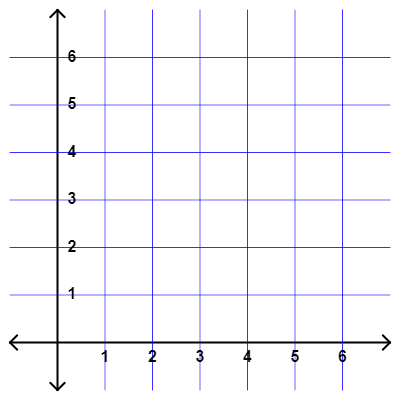
\includegraphics[width=.5\linewidth]{cartesian.png}
		      %	\caption{Logging and recovery}
		      \label{fig:recovery}
	      \end{figure}
	      \begin{itemize}
		      \item[(a)] \textbf{[1 point]} Draw a 6 by 6 space with all the 5 data points.
		      \item[(b)] \textbf{[3 points]} Estimate the model parameters $\theta$ and $\theta_0$.
		      \item[(c)] \textbf{[2 points]} Using~\eqref{eq:1}, argue that the least squares line,
		            \begin{equation}
			            y = \hat{\theta}x + \hat{\theta}_0,
		            \end{equation}
		            always passes through the points $(0,\hat{\theta}_0)$ and $(\bar{x},\bar{y})$,
		            where $\bar{x} = \tfrac{1}{5}\sum_{i=1}^{5}x_{i}$ and $\bar{y} = \tfrac{1}{5}\sum_{i=1}^{5} y_{i}$, and plot the line in the picture of (a).
		      \item[(d)] \textbf{[2 points]} Find the data point which makes the highest contribution to RSS, and show the geometric interpretation in the picture of (a).
		            %	\item[(e)] \textbf{[1 point]} Predict the output $\hat{y}_0$ of a testing data point $x_0 = 2.5$, and show it in the picture of (a). 

	      \end{itemize}

\end{enumerate}

\end{document}

